\section{Seleccionando voxels que ser\'an semillas}

Como ya dijimos, la materia gris est\'a compuesta principalmente por neuronas,
y la materia blanca por axones que las comunican. Como cada neurona
posee asociado un ax\'on, colocar semillas en la interfaz entre la materia gris
y la blanca permite caracterizar las neuronas de la corteza \cite{Mori2002}
\cite{Anwander2006}. Cibu et al. \cite{Thomas2014} muestran que la materia blanca
cercana a la materia gris est\'a interconectada por peque\~nos axones. Como
estamos interesados en realizar un estudio de las conexiones entre regiones
distantes del cerebro, decidimos situar las semillas a \textit{3mm} de la corteza,
evitando as\'i el efecto de \'estos axones locales. El problema es que la corteza
del cerebro no es uniforme, sino que est\'a llena de surcos y circunvoluciones. 
Calcular la distancia entonces no es inmediato, necesita un m\'etodo que tome
estas propiedades en cuenta. A continuaci\'on presentamos el m\'etodo
\textit{Fast Marching Method} y como es posible utilizarlo para posicionar las
semillas respetando la forma de la materia blanca. \\

\textit{Fast Marching Method} es un m\'etodo para resolver num\'ericamente una
versi\'on restringida de la ecuaci\'on \textit{Eikonal}. La misma, en su forma
general, es una ecuaci\'on diferencial no lineal que se encuentra com\'unmente 
en problemas de propagaci\'on de onda. Tiene la forma: 

$$ V(x) | \nabla u(x) | = F(x) , x \in \Omega $$ 

Donde $\Omega$ es un subconjunto abierto de $R^n$ con un
\textit{buen comportamiento} en su borde. $F(x)$ se denomina el costo temporal y
$V(x)$ es la velocidad de la onda en cada punto. En el caso particular que
queremos resolver $u(x_\omega) = 0, x \in \delta\Omega$;  $F(x)=1$ y $V(x)=1$,
por lo que la ecuaci\'on se resume a:

$$ | \nabla u(x) | = 1 , x \in \Omega $$ 

$u(v)$ en este caso representa el tiempo que tarda la onda en llegar desde
alg\'un elemento del borde hasta el punto $v$ movi\'endose a velocidad constante
de una unidad de espacio por unidad de tiempo. Dada la forma de la velocidad, 
$u(v)$ tambi\'en representa \textbf{la distancia mas corta que existe entre cualquier
punto $v$ de la imagen y el borde de $\Omega$}. Dependiendo la orientaci\'on que 
se elija, las distancias a los puntos internos de la superficie ser\'an negativas
y las distancias a los puntos externos positivas (Figura \ref{fig:fmm}). 
\textit{FMM} resuelve este problema en tiempo $O(n log(n))$ \cite{Sethian2001},
siendo $n$ la cantidad de voxels de la imagen.\\

\begin{figure}[h!]

\centering
\begin{minipage}[b]{0.7\textwidth}
    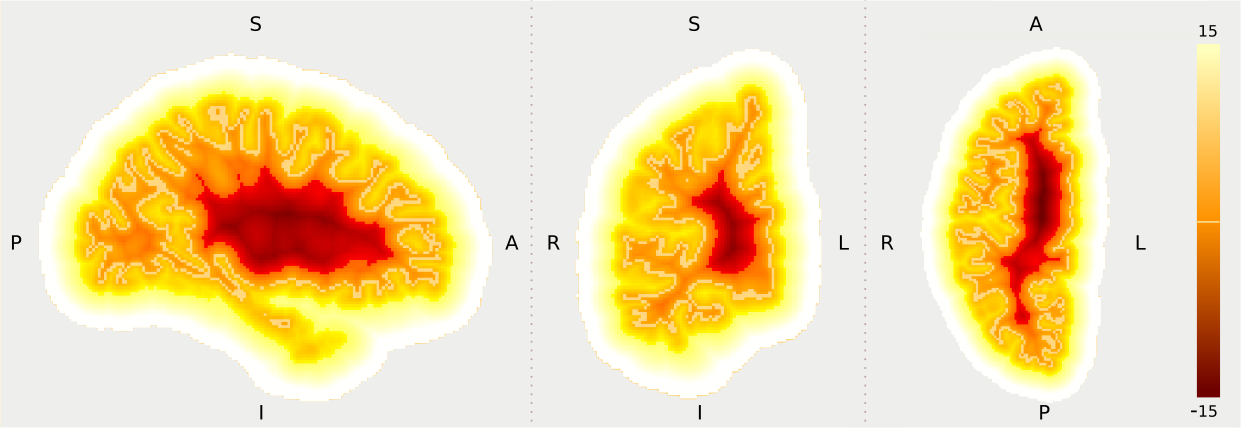
\includegraphics[width=\textwidth]{img/fmm.png}
    \caption{\small FMM sobre el hemisferio derecho, el borde la materia blanca fue
    resaltado intensionalmente}
    \label{fig:fmm}
\end{minipage} ~

\end{figure}  

Es posible utilizar este algoritmo para seleccionar voxels a cierta profundidad
en la materia blanca. Usando como borde la corteza cerebral podemos crear un mapa
de distancias en la materia blanca. El gradiente de este mapa de distancias es un
campo vectorial donde cada vector apunta hacia el interior de la materia blanca.
Caminar partiendo desde los puntos en la siguiendo este campo permite adentrarse 
respetando la morfolog\'ia de la materia blanca. Una ventaja de este m\'etodo es
que permite guardar un mapeo entre cada coordenada de la superficie y la semilla
que la representa. Otra ventaja es que es posible realizar todo el proceso en tiempo
$O(n log(n))$. \\
